\section{Erstes Bonusfeature: Audio-Ingame}\label{sec:audio-ingame}
Mit dem Kunden wurde als erstes Bonusfeature vereinbart, dass das Abspielen von Audio-Titeln in der Anwendung als Dauerschleife ermöglicht wird. 
Die Audio-Titel werden von dem Team 'Magical Studios' bereitgestellt, die zur jeweiligen Spielsituation und zum momentanen Bildschirm angepasst sind.
Dafür werden in den verschiedenen Bildschirmen verschiedene Audio-Titel abgespielt, die in der Tabelle~\ref{tab:audio} zu finden sind.
\subsection{Mockups}\label{subsec:mockups-audio-ingame}
Das Pausemenü wird in diesem Release mit dem 'Einstellungsmenü'-Knopf erweitert.
Das Fenster aus der Abbildung~\ref{fig: Pausemenü} erscheint, wenn der Nutzer auf den Knopf 'Pause' im Spielbildschirm drückt. 
Dabei ist wie in der Abbildung~\ref{fig: Pausemenü} der Knopf zum Fortsetzen des Spiels an erster Stelle, der Knopf zum Gelangen zum Einstellungsmenü an zweiter Stelle und der Knopf zum Verlassen des Spiels an letzter Stelle positioniert.
Beim Drücken des 'Einstellungsmenü'-Knopfs wird das Fenster aus der Abbildung~\ref{fig: Pausemenü} mit dem Fenster aus der Abbildung~\ref{fig: Einstellungsmenü} ersetzt. 
In diesem Fenster sind vier Knöpfe angezeigt: drei Knöpfe zum Öffnen der Ton-, Tastenkürzel- und Trainereinstellungen und ein Knopf zum Zurückkehren zum Pausemenü. Beim Drücken des 'Go Back'-Knopfs wird das Pausemenü erneut angezeigt.
Beim Öffnen der Toneinstellungen erscheint ein neues Fenster wie in Abbildung~\ref{fig: Audio-Einstellungen}, in dem eine Beschriftung für das Fenster, ein Schieberegler für die Verwaltung der Lautstärke und ein Knopf zum Schließen der Einstellungen beinhaltet sind. Beim Schließen der Einstellungen gelangt der Nutzer wieder zum Fenster aus Abbildung~\ref{fig: Einstellungsmenü}.
\begin{figure}[H]
    \center
    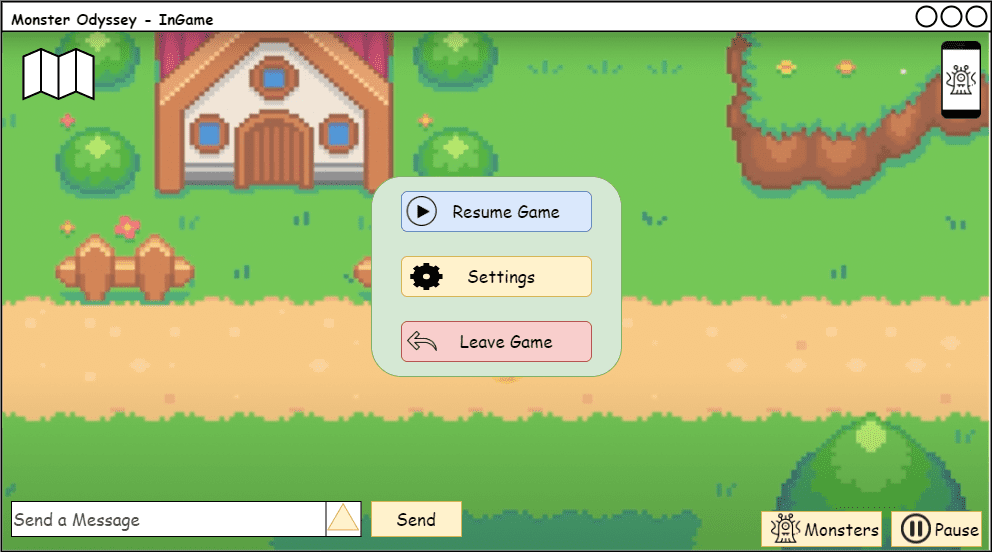
\includegraphics[scale=\scale]{images/mockups/Bonusfeatures/AudioIngame/IngameSettings.png}
    \caption{Mockup: Pausemenü}
    \label{fig: Pausemenü}
\end{figure}
\begin{figure}[H]
    \center
    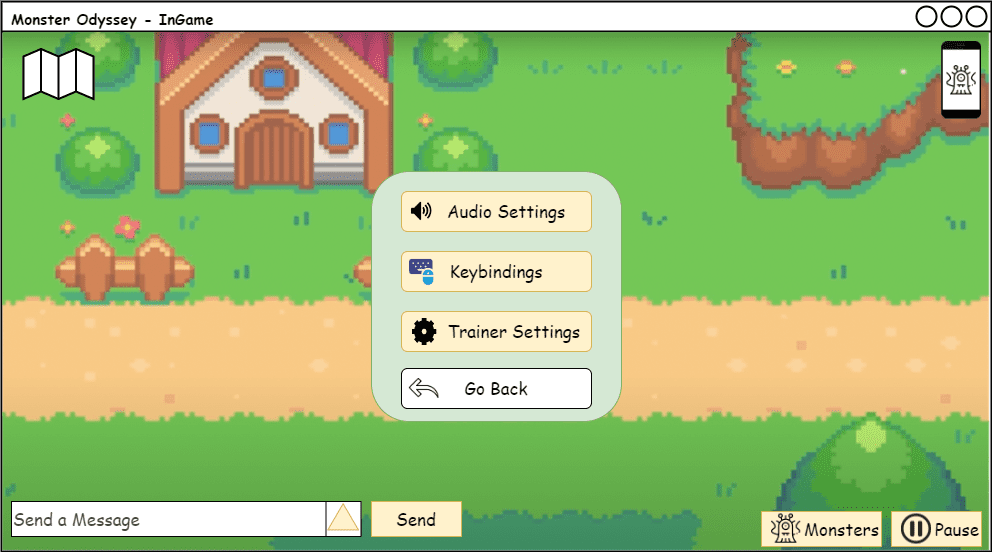
\includegraphics[scale=\scale]{images/mockups/Bonusfeatures/AudioIngame/IngameSettingsMenu.png}
    \caption{Mockup: Einstellungsmenü}
    \label{fig: Einstellungsmenü}
\end{figure}
\begin{figure}[H]
    \center
    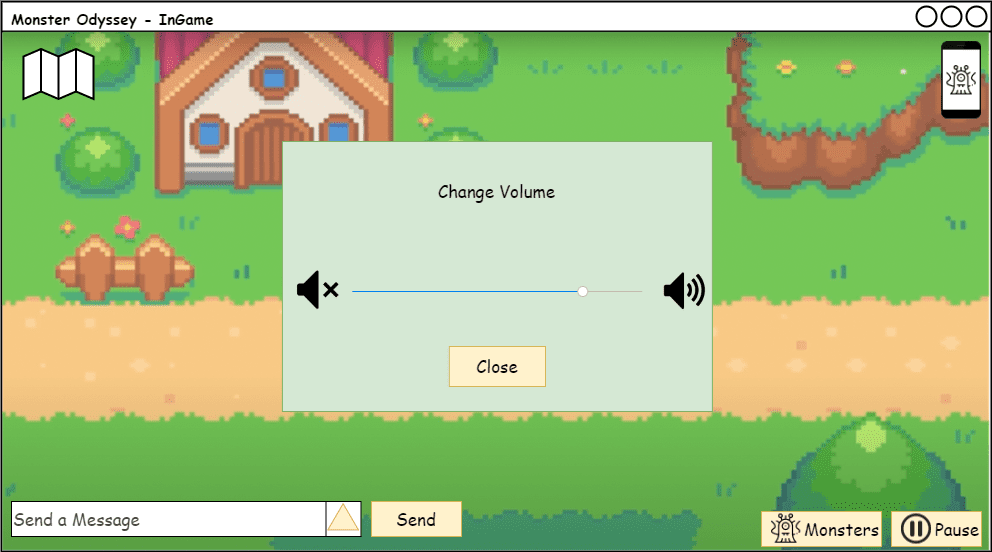
\includegraphics[scale=\scale]{images/mockups/Bonusfeatures/AudioIngame/AudioSettings.png}
    \caption{Mockup: Audio-Einstellungen}
    \label{fig: Audio-Einstellungen}
\end{figure}
Damit der Nutzer die Kontrolle über den Ton außerhalb des Spielbildschirms hat, sind zwei Knöpfe im Mainmenü- und Login-Bildschirm hinterlegt. Mithilfe dieser Knöpfe kann der Ton stummgeschaltet beziehungsweise die Stummschaltung aufgehoben werden. In der Abbildung~\ref{fig: Login-Bildschirm Audio-Knopf} wird der Knopf zum Stummschalten des Tons gedrückt. Hierdurch verwandelt wie in Abbildung~\ref{fig: Login-Bildschirm Audio-Knopf stumm} das Symbol, um mit dem aktuellen Status des Tons übereinzustimmen.
\begin{figure}[H]
    \centering
    \begin{subfigure}[b]{0.4\textwidth}
        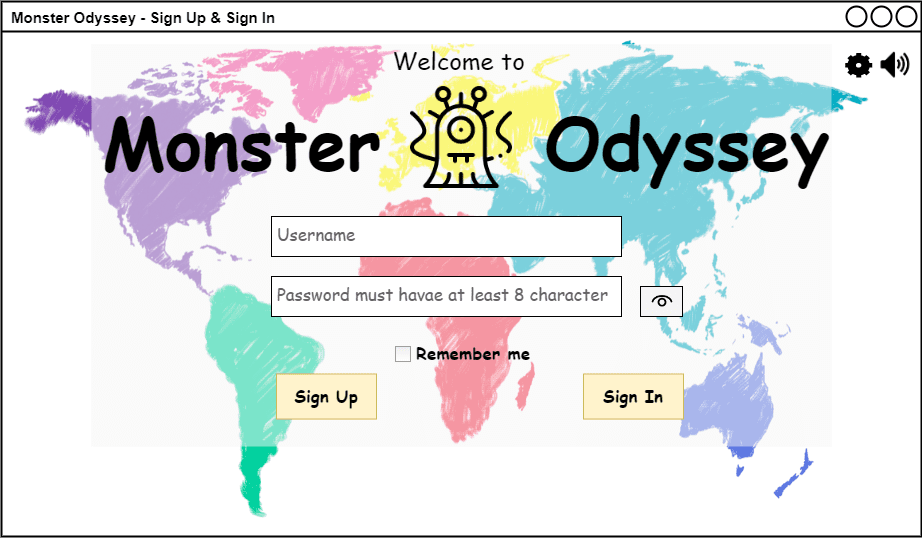
\includegraphics[width=\textwidth]{images/mockups/Bonusfeatures/AudioIngame/Login.png}
        \caption{Login-Bildschirm Audio-Knopf}
        \label{fig: Login-Bildschirm Audio-Knopf}
    \end{subfigure}
    \hfill
    \begin{subfigure}[b]{0.4\textwidth}
        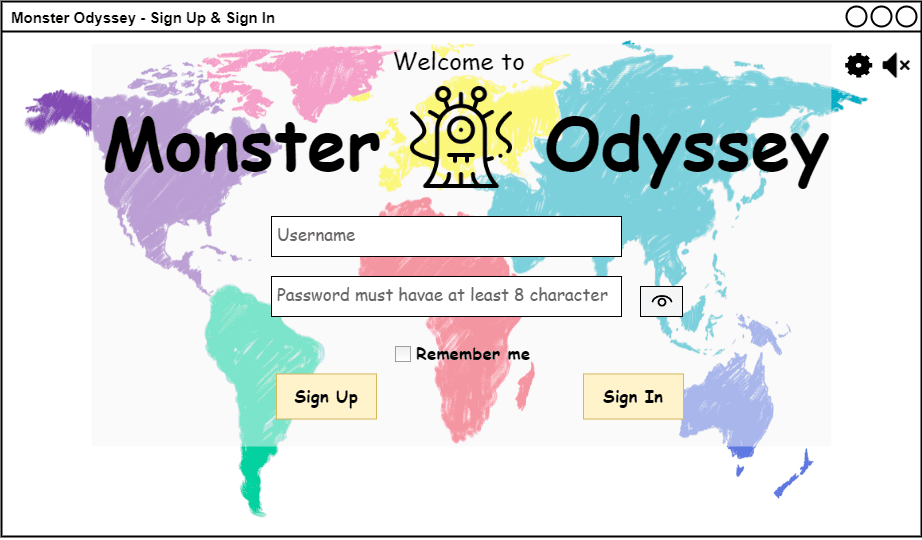
\includegraphics[width=\textwidth]{images/mockups/Bonusfeatures/AudioIngame/LoginMuted.png}
        \caption{Login-Bildschirm Audio-Knopf stumm}
        \label{fig: Login-Bildschirm Audio-Knopf stumm}
    \end{subfigure}
    \caption{Mockup: Login-Bildschirm}
    \label{fig: Login-Bildschirm}
\end{figure}
\subsection{Vergleich zwischen Mockups und Implementierung}\label{subsec:vergleich-zwischen-mockups-und-implementierung-audio-ingame}
Der einzig wesentliche Unterschied bei der Umsetzung dieser Anforderung ist, dass der Schieberegler für die Audio-Einstellungen in der Abbildung~\ref{fig: Implementierung: Audio-Einstellungen} etwas größer als in der Abbildung~\ref{fig: Mockup: Audio-Einstellungen} gestaltet ist. Dieser Unterschied ist  darauf zurückzuführen, dass sich das Konzipieren des Schiebereglers schwieriger als erwartet herausgestellt hat und aufgrund von Zeitprobleme weggelassen worden ist.
\begin{figure}[H]
    \centering
    \begin{subfigure}[b]{0.4\textwidth}
        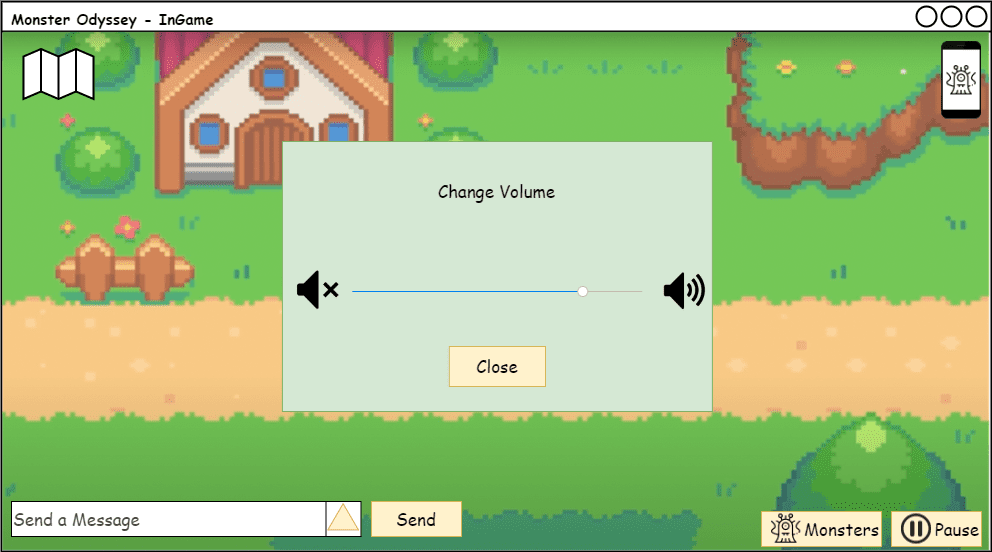
\includegraphics[width=\textwidth]{images/mockups/Bonusfeatures/AudioIngame/AudioSettings.png}
        \caption{Mockup: \phantom{aaa} Audio-Einstellungen}
        \label{fig: Mockup: Audio-Einstellungen}
    \end{subfigure}
    \hfill
    \begin{subfigure}[b]{0.4\textwidth}
        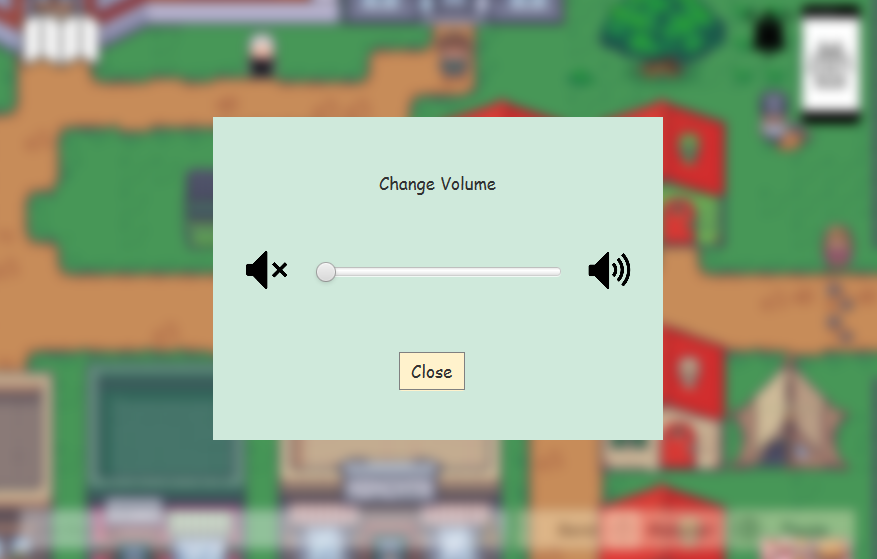
\includegraphics[width=\textwidth]{images/implementation/Bonusfeatures/AudioIngame/audioingameimp.PNG}
        \caption{Implementierung: Audio-Einstellungen}
        \label{fig: Implementierung: Audio-Einstellungen}
    \end{subfigure}
    \caption{Vergleich: Bonusfeature Audio im Spiel}
    \label{fig: Vergleich: Bonusfeature Audio im Spiel}
\end{figure}
Des Weiteren ist in den Abbildungen~\ref{fig: Vergleich: Pausemenü} und~\ref{fig: Vergleich: Einstellungsmenü} anzumerken, dass die Implementierungen mit den Mockups für das Pause-/Einstellungsmenü identisch sind. 
\begin{figure}[H]
    \centering
    \begin{subfigure}[b]{0.4\textwidth}
        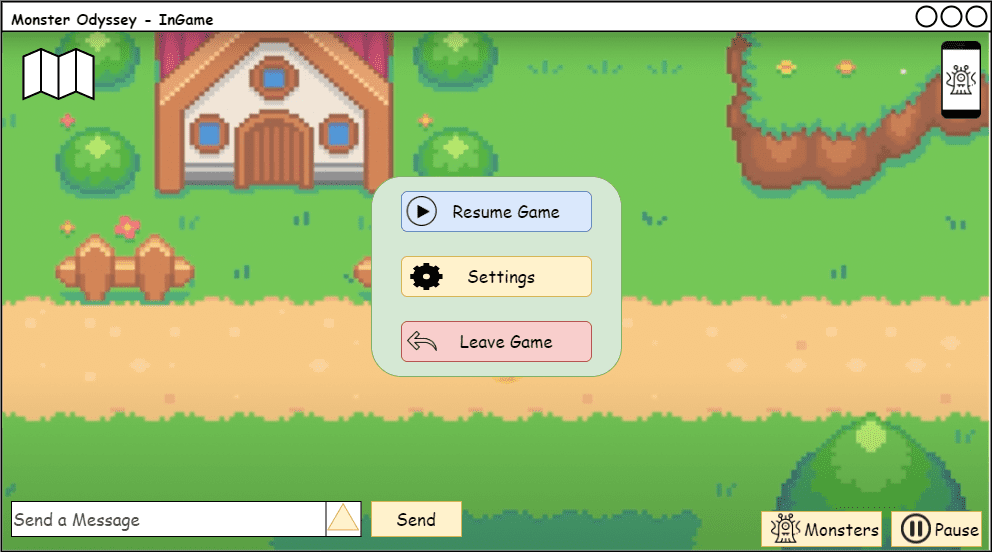
\includegraphics[width=\textwidth]{images/mockups/Bonusfeatures/AudioIngame/IngameSettings.png}
        \caption{Mockup: Pausemenü}
        \label{fig: Mockup: Pausemenü}
    \end{subfigure}
    \hfill
    \begin{subfigure}[b]{0.4\textwidth}
        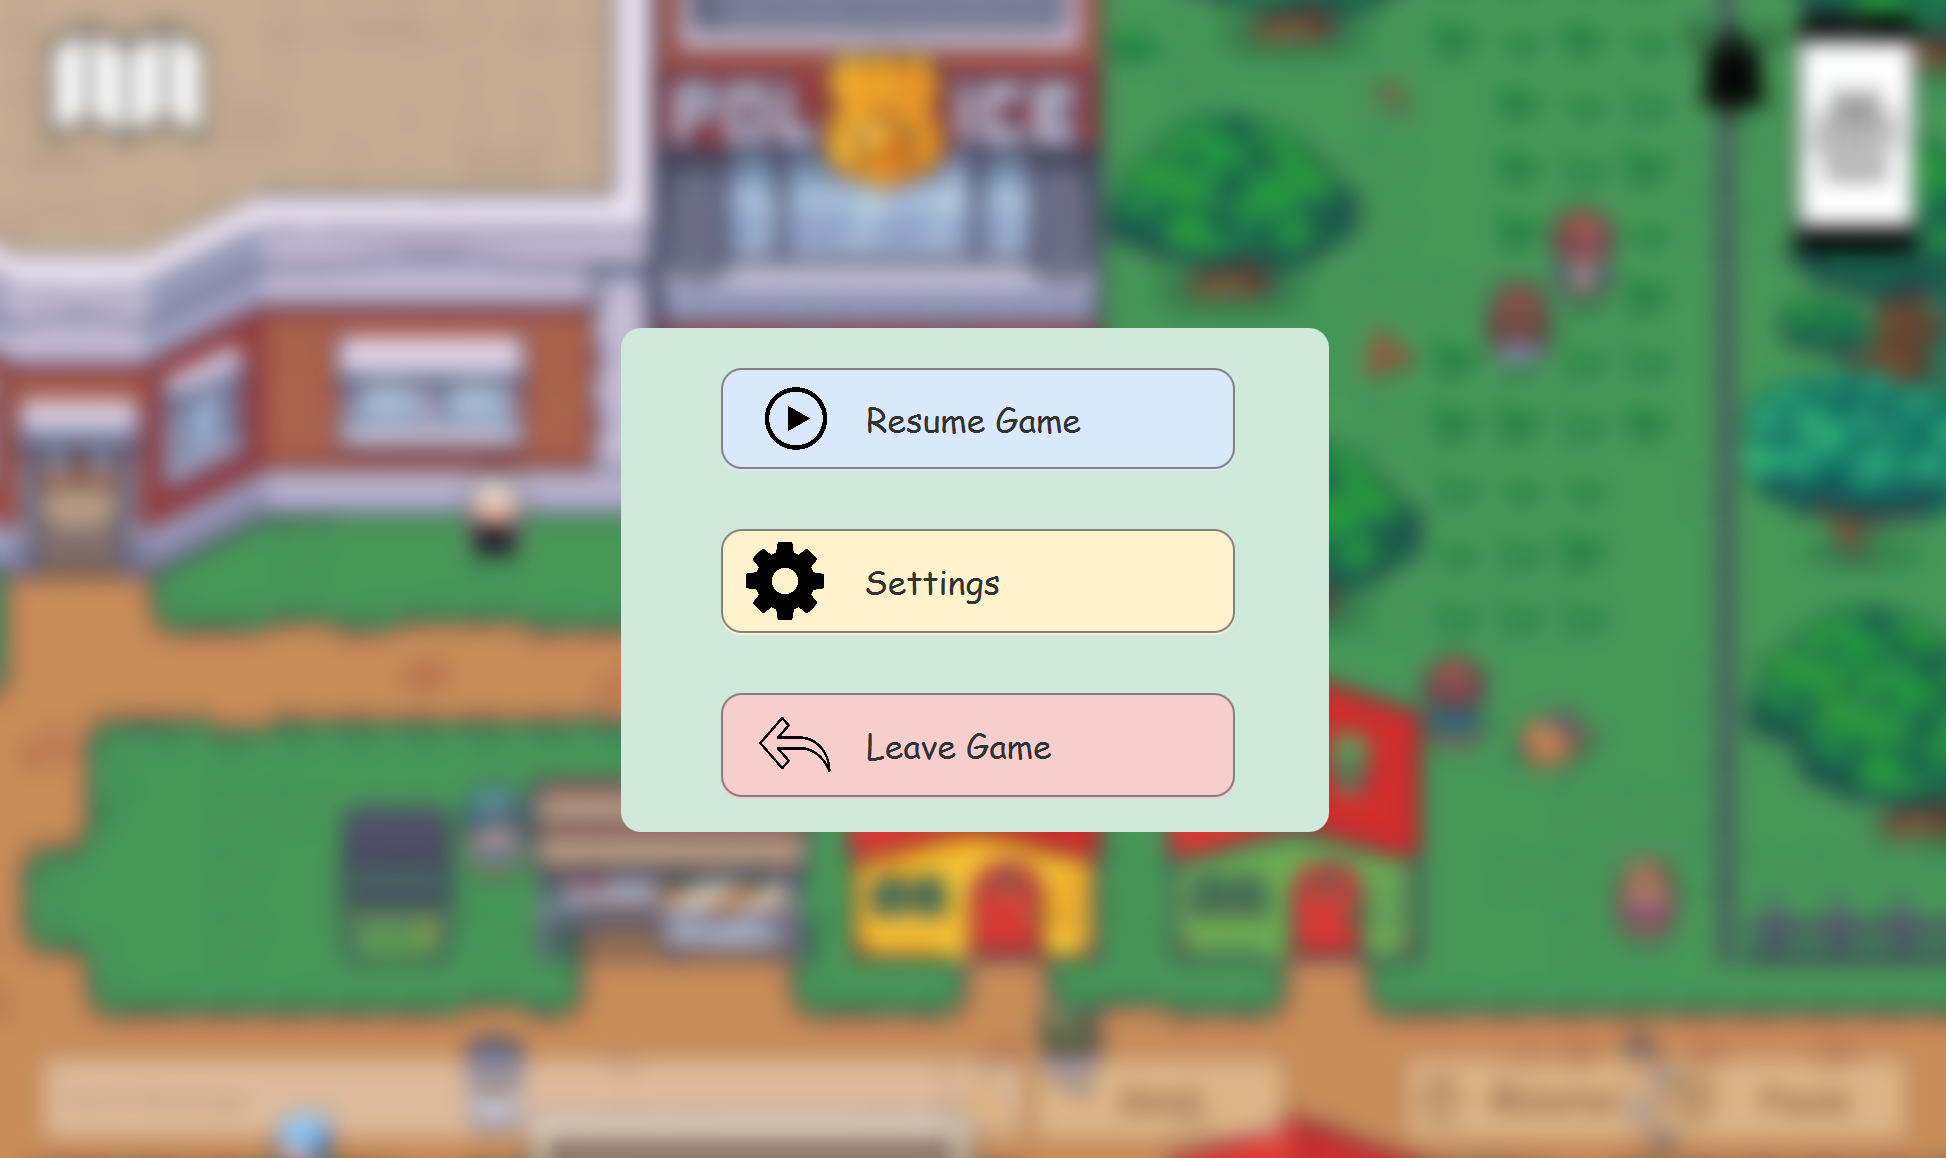
\includegraphics[width=\textwidth]{images/implementation/Bonusfeatures/AudioIngame/Pausemenu imp.png}
        \caption{Implementierung: Pausemenü}
        \label{fig: Implementierung: Pausemenü}
    \end{subfigure}
    \caption{Vergleich: Pausemenü}
    \label{fig: Vergleich: Pausemenü}
\end{figure}
\begin{figure}[H]
    \centering
    \begin{subfigure}[b]{0.4\textwidth}
        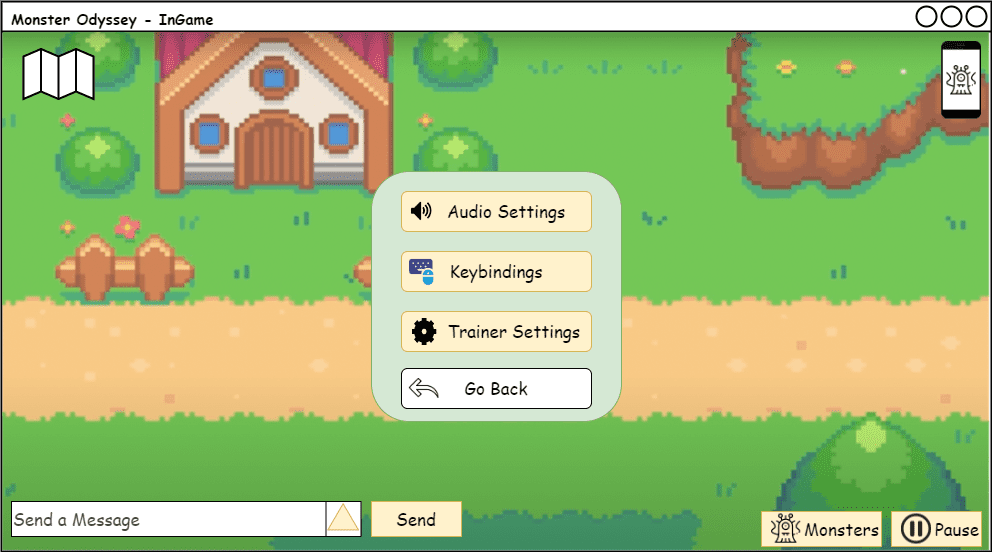
\includegraphics[width=\textwidth]{images/mockups/Bonusfeatures/AudioIngame/IngameSettingsMenu.png}
        \caption{Mockup: ~\phantom{aaaaaa} Einstellungsmenü}
        \label{fig: Mockup: Einstellungsmenü}
    \end{subfigure}
    \hfill
    \begin{subfigure}[b]{0.4\textwidth}
        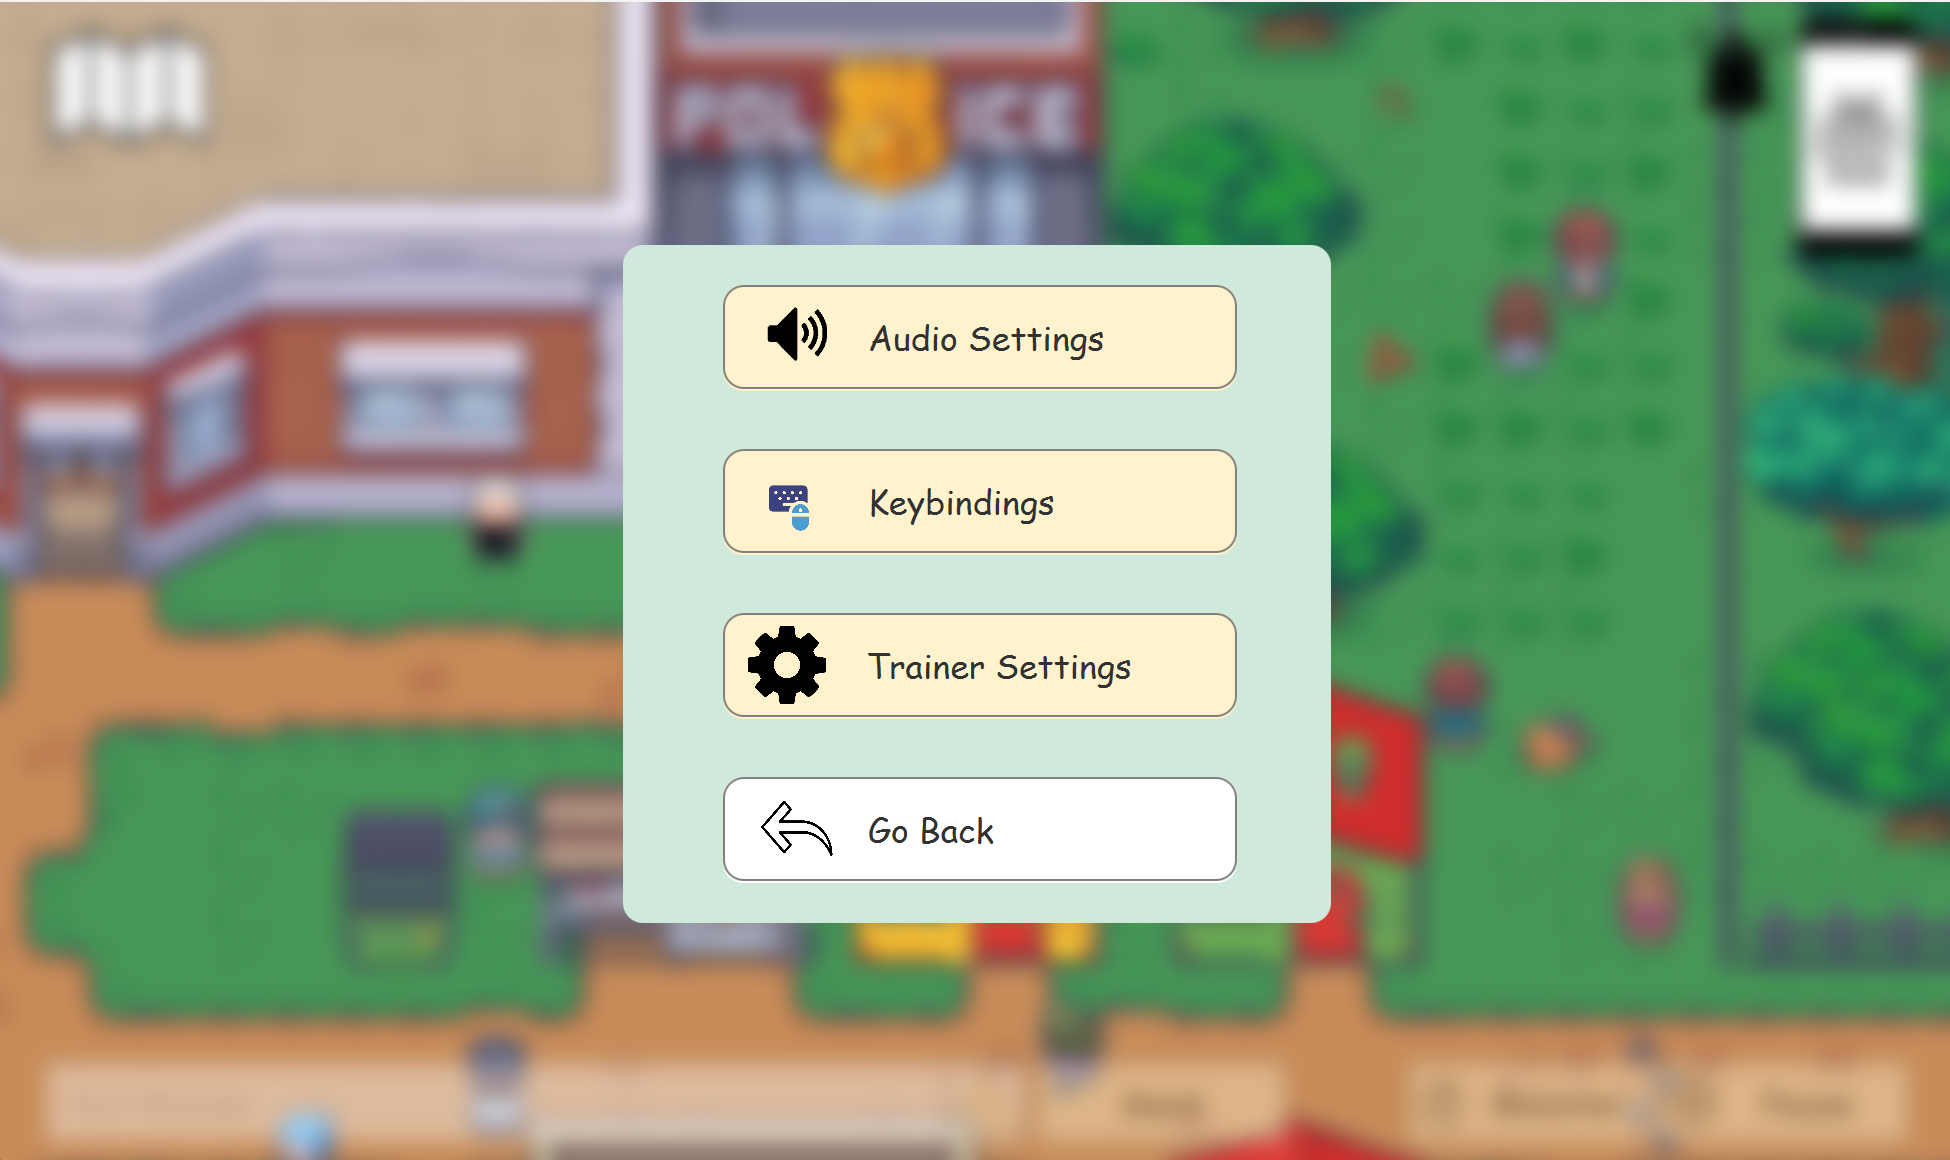
\includegraphics[width=\textwidth]{images/implementation/Bonusfeatures/AudioIngame/Settingsmenu imp.png}
        \caption{Implementierung: Einstellungsmenü}
        \label{fig: Implementierung: Einstellungsmenü}
    \end{subfigure}
    \caption{Vergleich: Einstellungsmenü}
    \label{fig: Vergleich: Einstellungsmenü}
\end{figure}